\documentclass[
  shownotes,
  xcolor={svgnames},
  hyperref={colorlinks,citecolor=DarkBlue,linkcolor=DarkRed,urlcolor=DarkBlue}
  ]{beamer}
\usepackage{animate}
\usepackage{amsmath}
\usepackage{amsfonts}
\usepackage{amssymb}
\usepackage{pifont}
\usepackage{mathpazo}
%\usepackage{xcolor}
\usepackage{multimedia}
\usepackage{fancybox}
\usepackage[para]{threeparttable}
\usepackage{multirow}
\setcounter{MaxMatrixCols}{30}
\usepackage{subcaption}
\usepackage{graphicx}
\usepackage{lscape}
\usepackage[compatibility=false,font=small]{caption}
\usepackage{booktabs}
\usepackage{ragged2e}
\usepackage{chronosys}
\usepackage{appendixnumberbeamer}
\usepackage{animate}
\setbeamertemplate{caption}[numbered]
\usepackage{color}
%\usepackage{times}
\usepackage{tikz}
\usepackage{comment} %to comment
%% BibTeX settings
\usepackage{natbib}
\bibliographystyle{apalike}
\bibpunct{(}{)}{,}{a}{,}{,}
\setbeamertemplate{bibliography item}{[\theenumiv]}

% Defines columns for bespoke tables
\usepackage{array}
\newcolumntype{L}[1]{>{\raggedright\let\newline\\\arraybackslash\hspace{0pt}}m{#1}}
\newcolumntype{C}[1]{>{\centering\let\newline\\\arraybackslash\hspace{0pt}}m{#1}}
\newcolumntype{R}[1]{>{\raggedleft\let\newline\\\arraybackslash\hspace{0pt}}m{#1}}


\usepackage{xfrac}


\usepackage{multicol}
\setlength{\columnsep}{0.5cm}

% Theme and colors
\usetheme{Boadilla}

% I use steel blue and a custom color palette. This defines it.
\definecolor{andesred}{HTML}{af2433}

% Other options
\providecommand{\U}[1]{\protect\rule{.1in}{.1in}}
\usefonttheme{serif}
\setbeamertemplate{itemize items}[default]
\setbeamertemplate{enumerate items}[square]
\setbeamertemplate{section in toc}[circle]

\makeatletter

\definecolor{mybackground}{HTML}{82CAFA}
\definecolor{myforeground}{HTML}{0000A0}

\setbeamercolor{normal text}{fg=black,bg=white}
\setbeamercolor{alerted text}{fg=red}
\setbeamercolor{example text}{fg=black}

\setbeamercolor{background canvas}{fg=myforeground, bg=white}
\setbeamercolor{background}{fg=myforeground, bg=mybackground}

\setbeamercolor{palette primary}{fg=black, bg=gray!30!white}
\setbeamercolor{palette secondary}{fg=black, bg=gray!20!white}
\setbeamercolor{palette tertiary}{fg=white, bg=andesred}

\setbeamercolor{frametitle}{fg=andesred}
\setbeamercolor{title}{fg=andesred}
\setbeamercolor{block title}{fg=andesred}
\setbeamercolor{itemize item}{fg=andesred}
\setbeamercolor{itemize subitem}{fg=andesred}
\setbeamercolor{itemize subsubitem}{fg=andesred}
\setbeamercolor{enumerate item}{fg=andesred}
\setbeamercolor{item projected}{bg=gray!30!white,fg=andesred}
\setbeamercolor{enumerate subitem}{fg=andesred}
\setbeamercolor{section number projected}{bg=gray!30!white,fg=andesred}
\setbeamercolor{section in toc}{fg=andesred}
\setbeamercolor{caption name}{fg=andesred}
\setbeamercolor{button}{bg=gray!30!white,fg=andesred}

\makeatother


%%%%%%%%%%%%%%% BEGINS DOCUMENT %%%%%%%%%%%%%%%%%%

\begin{document}

\title[Lecture 2]{Lecture 2: \\ The classic paradigm \\ vs \\ the predictive paradigm}
\subtitle{Big Data and Machine Learning for Applied Economics \\ Econ 4676}
\date{\today}

\author[Sarmiento-Barbieri]{Ignacio Sarmiento-Barbieri}
\institute[Uniandes]{Universidad de los Andes}


\begin{frame}[noframenumbering]
\maketitle
\end{frame}

%%%%%%%%%%%%%%%%%%%%%%%%%%%%%%%%%%%
%       Motivation              %
% What is the question?
% Why do we care?
% What is new?
% What do you find?
%%%%%%%%%%%%%%%%%%%%%%%%%%%%%%%%%%%




\begin{frame}
\frametitle{Agenda}

\tableofcontents


\end{frame}



%%----------------------------------------------------------------------%

\section{Motivation}
\begin{frame}
\frametitle{Recap Last Class}


{\bf Motivation}

\bigskip

\begin{itemize}
      \item We discussed the examples of Google Flu and Facebook face detection
      \medskip
      \begin{itemize}
        \item Take away, the success was driven by an empiric approach
        \item Given data  estimate a function $f(x)$ that predicts $y$ from $x$
      \end{itemize}
      \medskip
      
      \item  This is basically what we do as economists everyday so: 
      \begin{itemize}
        \item  Are these algorithms merely applying standard techniques to novel and large datasets? 
        \item  If there are fundamentally new empirical tools, how do they fit with what we know? 
        \item  As empirical economists, how can we use them? 
       \end{itemize}
\end{itemize}

\end{frame}


%----------------------------------------------------------------------%
\section{The Classic Paradigm}
\begin{frame}
\frametitle{The Classic Paradigm}


\begin{align}
Y=f(X)+u
\end{align}
\medskip
\begin{itemize}
  \item Interest lies on inference 
  \medskip
  \item "Correct" $f()$ to understand how Y is affected by X
  \medskip
  \item Model: Theory, experiment
  \medskip
  \item Hypothesis testing (std. err., tests)
\end{itemize}

\end{frame}

%----------------------------------------------------------------------%
\begin{frame}
\frametitle{Example: OLS and the classical model}

Set 

\begin{align}
f(X)=X\beta
\end{align}

\begin{itemize}
    \item $Y=X\beta+u$ 
    \item Interest in $\beta$

    \item The model is given. 
    \item Problem: how to estimate $\beta$ in the given model?
    \item Minimize $SSR$
      \begin{align}
          \hat \beta= (X'X)^{-1} X'y
      \end{align}


    \item Gauss-Markov: under the classical assumptions it is BLUE

    \item Classical assumptions: how they affect properties (omitted variables, endogeneity, heteroscedasticity, etc.)
\end{itemize}

\end{frame}

%----------------------------------------------------------------------%

\begin{frame}
\frametitle{The Predictive Paradigm}


\begin{align}
Y=f(X)+u
\end{align}

\begin{itemize}
  \item Interest on predicting $Y$
  \medskip
  \item "Correct" $f()$ to be able to predict (no inference!)
  \medskip
  \item Model? 
  
\end{itemize}


\end{frame}


%----------------------------------------------------------------------%
\section{Statistical Decision Theory}
\begin{frame}
\frametitle{Statistical Decision Theory: A bit of theory}

\begin{itemize}
  \item We need a bit of theory to give us a framework for choosing $f$
  \item A decision theory approach involves an {\bf action space} $\mathcal{A}$
  \item The {\bf action space} $\mathcal{A}$ specify the possible "actions we might take"
  \item Some examples
\end{itemize}

\footnotesize

\begin{table}[H]
\caption{Action Spaces}

\begin{centering}
\begin{tabular}{cc}
\hline 
Inference & Action Space\\
\hline 
\hline 
Estimation $\theta$, $g\left(\theta\right)$  & $\mathcal{A}=\Theta$\\
Prediction & $\mathcal{A}=space\,of\,X_{n+1}$\\
Model Selection & $\mathcal{A}=\left\{ Model\,I,Model\,II,...\right\} $\\
Hyp. Testing & $\mathcal{A}=\left\{ Reject|Accept\,H_{0}\right\} $\\

\hline 
\end{tabular}
\par\end{centering}
\end{table}


\end{frame}

%----------------------------------------------------------------------%

\begin{frame}
\frametitle{Statistical Decision Theory: A bit of theory}


\begin{itemize}
  \item After the data $X=x$ is observed, where $X\sim f(X|\theta)$, $\theta \in \Theta$
  \item A decision is made
  \item The set of allowable decisions is the action space ($\mathcal{A}$)
  \item The loss function in an estimation problem reflects the fact that if an action $a$ is close to $\theta$,
  \begin{itemize}
   \item then the decision $a$ is reasonable and little loss is incurred.
   \item if it is far then a large loss is incurred
  \end{itemize}
\end{itemize}

\begin{align}
    L:\mathcal{A}\rightarrow\left[0,\infty\right]
\end{align}


\end{frame}
%----------------------------------------------------------------------%

\begin{frame}
\frametitle{Statistical Decision Theory: A bit of theory}
\framesubtitle{Loss Function}

\begin{itemize}
\item If $\theta$ is real valued, two of the most common loss functions are

\begin{itemize}
  \item Squared Error Loss:
  
  \begin{align}
      L(a,\theta)=(a-\theta)^{2}
  \end{align}
    
    \item Absolute Error Loss:

    \begin{align}
      L(a,\theta)=|a-\theta|
    \end{align}
\end{itemize}


\item These two are symmetric functions. However, there's no restriction. For example in hypothesis testing a "0-1" Loss is common.
\item Loss is minimum if the action is correct
\end{itemize}
%how $L$ looks as longs as it maps into $\left[0,\infty\right]$. 
\end{frame}
%----------------------------------------------------------------------%



\begin{frame}
\frametitle{Statistical Decision Theory: A bit of theory}
\framesubtitle{Risk Function}
In a decision theoretic analysis, the quality of an estimator is quantified by its risk function, that is, for an estimator $\delta(x)$ of $\theta$, the risk function is 

\begin{align}
      R(\theta,\delta)=E_\theta L(\theta,\delta(X))
    \end{align}

    at a given $\theta$, the risk function is the average loss that will be incurred if the estimator $\delta(X)$ is used


\begin{itemize}
\item since $\theta$ is unknown we would like to use an estimator that has a small value of $R(\theta,\delta)$ for all values $\theta$
\item Loss is minimum if the action is correct
\item If we need to compare two estimators ($\delta_1$ and $\delta_2$) then we will compare their risk functions
\item If $R(\delta_1,\theta)<R(\delta_2,\theta)$ for all $\theta \in \Theta$, then $\delta_1$ is preferred becasue it performs better for all $\theta$

\end{itemize}

\end{frame}
%----------------------------------------------------------------------%

\begin{comment}
\begin{frame}
\frametitle{Statistical Decision Theory: A bit of theory}
\framesubtitle{Risk Function}

\textbf{Frequentist Approach}

\[
E_{\theta}L\left(\delta\left(\underline{X}\right),\theta\right)=R\left(\delta,\theta\right)
\]

note that $\underline{X}$ are generated from a model with parameter
$\theta$.

\textbf{Bayesian Approach}

\[
E_{\theta}\left[L\left(\delta\left(\underline{X}\right),\theta\right)|\theta=\theta_{0}\right]=R\left(\delta,\theta_{0}\right)
\]

In the bayesian approach the data is generated from $\underline{X}|\theta=\theta_{0}$,
the parameter is not fixed, comes from a distribution.

\end{frame}
\end{comment}
%----------------------------------------------------------------------%
\begin{frame}
\frametitle{How to choose $f$ for prediction}
\begin{itemize}
  \item In a prediction problem we want to predict $Y$ from $f(X)$ in such a way that the loss is minimum
  \item Assume also that $X \in \mathbb{R}^p$ and $Y \in \mathbb{R}$ with joint distribution $Pr(X,Y)$
\end{itemize}

\begin{align}
  R(Y,f(X)) &=E[(Y-f(X)^2] \\
            &=\int (y-f(x)^2 Pr(dx,dy)
\end{align}

conditioning on X we have that
\begin{align}
 R(Y,f(X)|X) &= E_X E_{Y|X} [(Y-f(X))^2|X] 
\end{align}

this risk is also know as the {\bf mean squared (prediction) error} $Err(f)$
\end{frame}
%----------------------------------------------------------------------%

\begin{frame}
\frametitle{Mean square error}

It suffices to minimize  the $Err(f)$ point wise so

\begin{align}
f(x)= argmin_m E_{Y|X} [(Y-m)^2|X=x)
\end{align}

Y a random variable and m a constant (predictor)

\begin{align}
min_m E(Y-m)^2= \int (y-m)^2  f(y)dy 
\end{align}
Result: The best prediction of $Y$ at any point $X = x$ is the conditional mean, when best is measured by mean squared error. 

\end{frame}
%----------------------------------------------------------------------%

\begin{frame}
\frametitle{Mean square error}
Proof

FOC 

\begin{align}
\int -2 (y-m)  f(y)  dy =0 
\end{align}

Divided by -2 and clearing

\begin{align}
 m \int (y) dy = \int y f(y)  dz =0 
\end{align}
\begin{align}
m=E(Y|X=x) 
\end{align}


The best prediction of $Y$ at any point $X = x$ is the conditional mean, when best is measured by mean squared error.
\end{frame}
%----------------------------------------------------------------------%

\section{Reducible and Irreducible Error}
\begin{frame}
\frametitle{Reducible and Irreducible Error}



\begin{align}
  Y=f(X)+u 
\end{align}


\begin{itemize}
    \item  If $f$ were known and $X$ were observable, the problem comes down to predicting $u$
    \item  Given that $u$ is not observable, the best prediction in MSE is its expectation. $u$ is the irreducible error
    \item  When $f(.)$ is also unknown, the prediction problem is reduced to knowing $f(.)$
    \item  The 'reducible' error refers to the discrepancy between   $\hat f(.)$ and $f(.)$

\end{itemize}

\end{frame}
%----------------------------------------------------------------------%
\begin{frame}
\frametitle{Reducible and irreducible error}

\begin{itemize}
\item Let's think about our usual problem $f(.)$ is unknown
\item Consider a given estimate $\hat f$ and a set of predictors
\item this predictors yield $\hat Y = \hat f(x)$. 
\item For now assume $\hat f$ and X are fixed {\tiny (Hastie et al. make this assumption any idea why?)}
\item Then we can show that the mean square error
\end{itemize}

\begin{align}
E(Y-\hat Y)^2 &= E(f(X)+u - \hat f(X))^2 \\
      &= \underset{Reducible}{\underbrace{[f(X)-\hat{f}(X)]^{2}}}+\underset{Irreducible}{\underbrace{Var(u)}}
\end{align}

\end{frame}
%----------------------------------------------------------------------%
\begin{frame}
\frametitle{Reducible and irreducible error}

\begin{align}
E(Y-\hat Y)^2  &= \underset{Reducible}{\underbrace{[f(X)-\hat{f}(X)]^{2}}}+\underset{Irreducible}{\underbrace{Var(u)}}
\end{align}
\bigskip
\begin{itemize}
\item The focus the is on techniques for estimating $f$ with the aim of minimizing the reducible error
\medskip
\item It is important to keep in mind that the irreducible error will always provide an upper bound on the accuracy of our prediction for $Y$
\medskip
\item This bound is almost always unknown in practice
\end{itemize}

\end{frame}
%----------------------------------------------------------------------%

\begin{frame}
\frametitle{Variance Decomposition/ Bias}

Remember
\begin{itemize}
  \item $Bias (\hat f(X) )=E (\hat f(X) )-f=E (\hat f(X)-f(X))$
  \item  $Var (\hat f)  =E (\hat f - E (\hat f))^2$
\end{itemize}  

\bigskip
{\bf Result} (very important!)
\bigskip

\begin{align}
  MSE = Bias^2 (\hat f(X))+V (\hat f(X)) 
\end{align}

{\tiny Proof: as an exercise}

\end{frame}
%----------------------------------------------------------------------%

\begin{frame}
\frametitle{The econometric approach}

\begin{align}
MSE = Bias^2 (\hat f(X))+V (\hat f(X)) 
\end{align}

\bigskip

\begin{itemize}
  \item  When $\hat f(X)$ is unbiased, minimize MSE $\hat f(X)$ is reduced to minimize  $V(\hat f(X))$
  \medskip
  \item The best kept secret: tolerating some bias is possible to reduce V($\hat f(X)$) and lower MSE
  \medskip
  \item  If the goal is to predict, it is not a problem to tolerate biased estimates
  \medskip
  \item  It could be the case that the MSE is minimum for biased predictors
\end{itemize}
\end{frame}


%----------------------------------------------------------------------%

\begin{frame}<1>[label=estimate_f]
\frametitle{How to estimate $f()$}


\begin{itemize}
  \item Parametric methods $\rightarrow$ assume the functional form $\rightarrow$ from economic theory?
  \pause
  \medskip
  \item Non-Parametric methods $\rightarrow$ no assumption about $f()$ let the data speak
    
\end{itemize}

\end{frame}



%----------------------------------------------------------------------%

\begin{frame}
\frametitle{How to estimate $f(.)$}




\begin{figure}[H] \centering
  \centering
  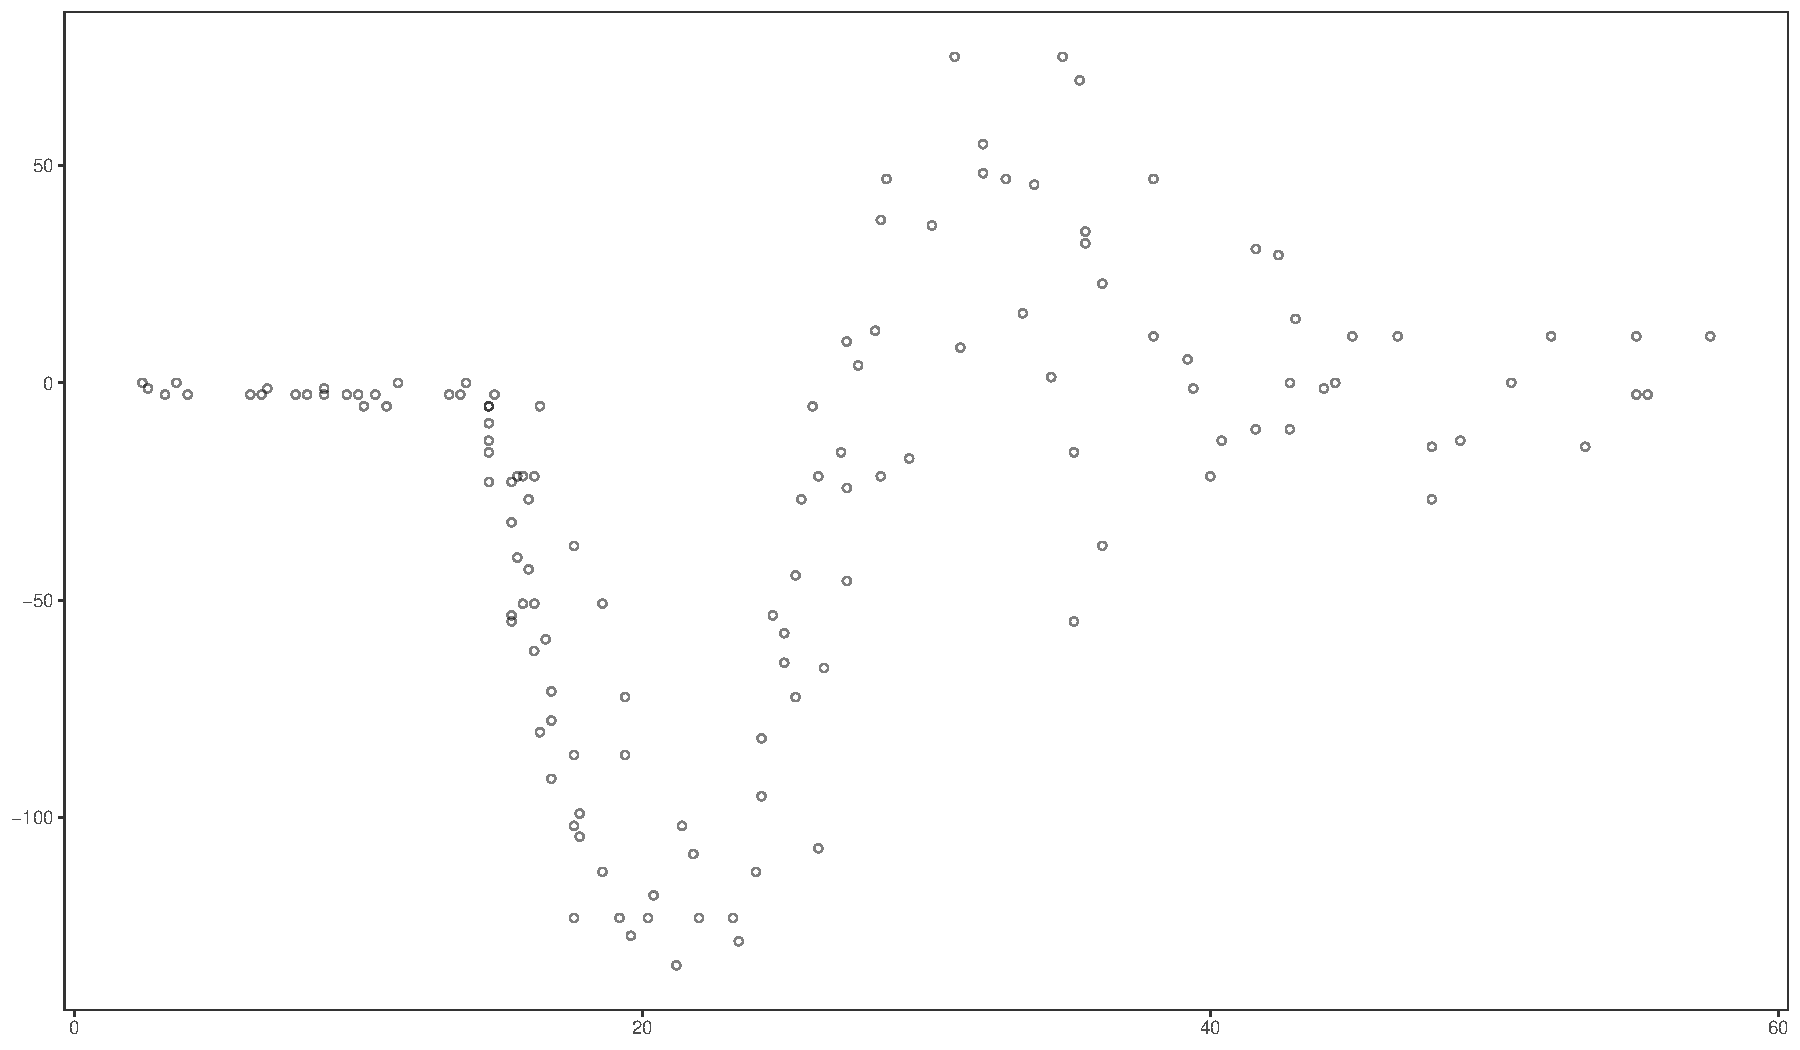
\includegraphics[scale=0.25]{figures/fig_1.pdf}
  \\
  \tiny
  Source: motorcycle data from \url{https://www.stata-press.com/data/r12/r.html}
\end{figure}


\end{frame}

%----------------------------------------------------------------------%

\begin{frame}
\frametitle{How to estimate $f(.)$}


\begin{itemize}
  \item Linear $f(X)=X\beta$
\end{itemize}

\begin{figure}[H] \centering
  \centering
  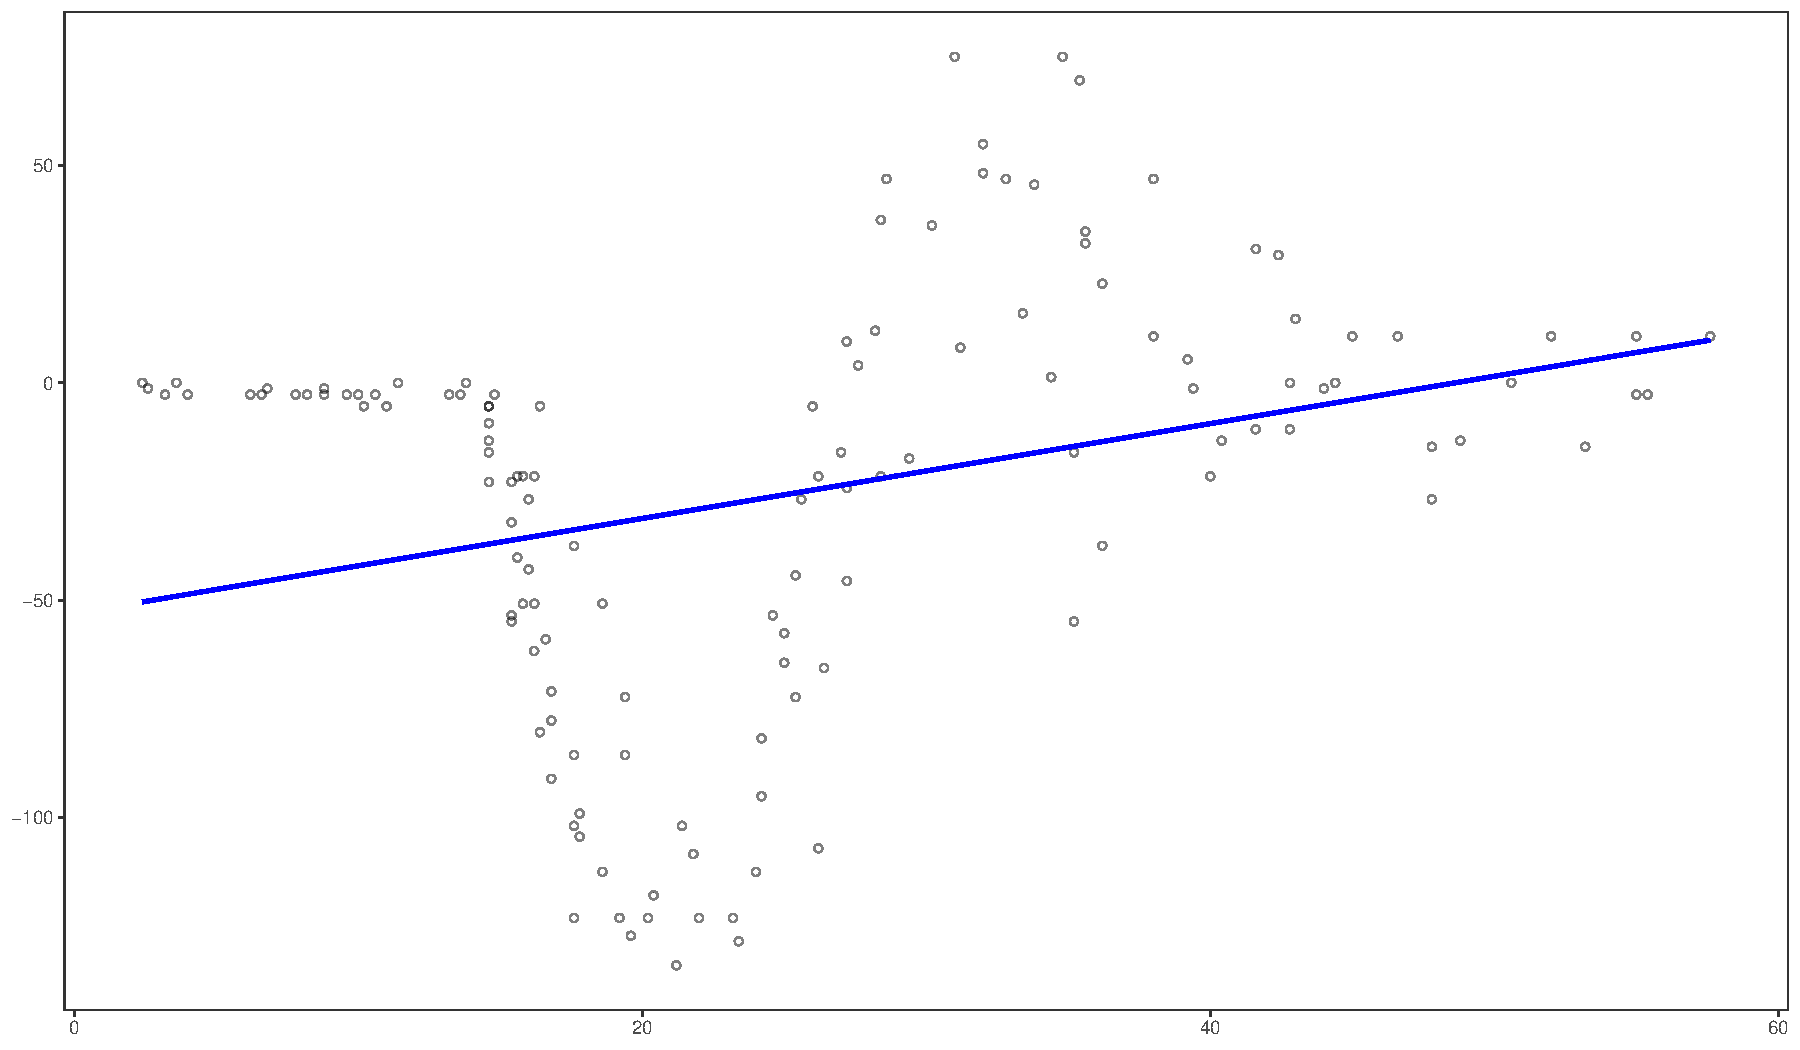
\includegraphics[scale=0.25]{figures/fig_1b.pdf}
  \\
  \tiny
  Source: motorcycle data from \url{https://www.stata-press.com/data/r12/r.html}
\end{figure}

\end{frame}

%----------------------------------------------------------------------%
%----------------------------------------------------------------------%
\againframe<2>{estimate_f}
%----------------------------------------------------------------------%
%----------------------------------------------------------------------%

\begin{frame}
\frametitle{How to estimate $f(.)$}


\begin{itemize}
  \item Local Polynomial Regression
\end{itemize}

\begin{figure}[H] \centering
  \centering
  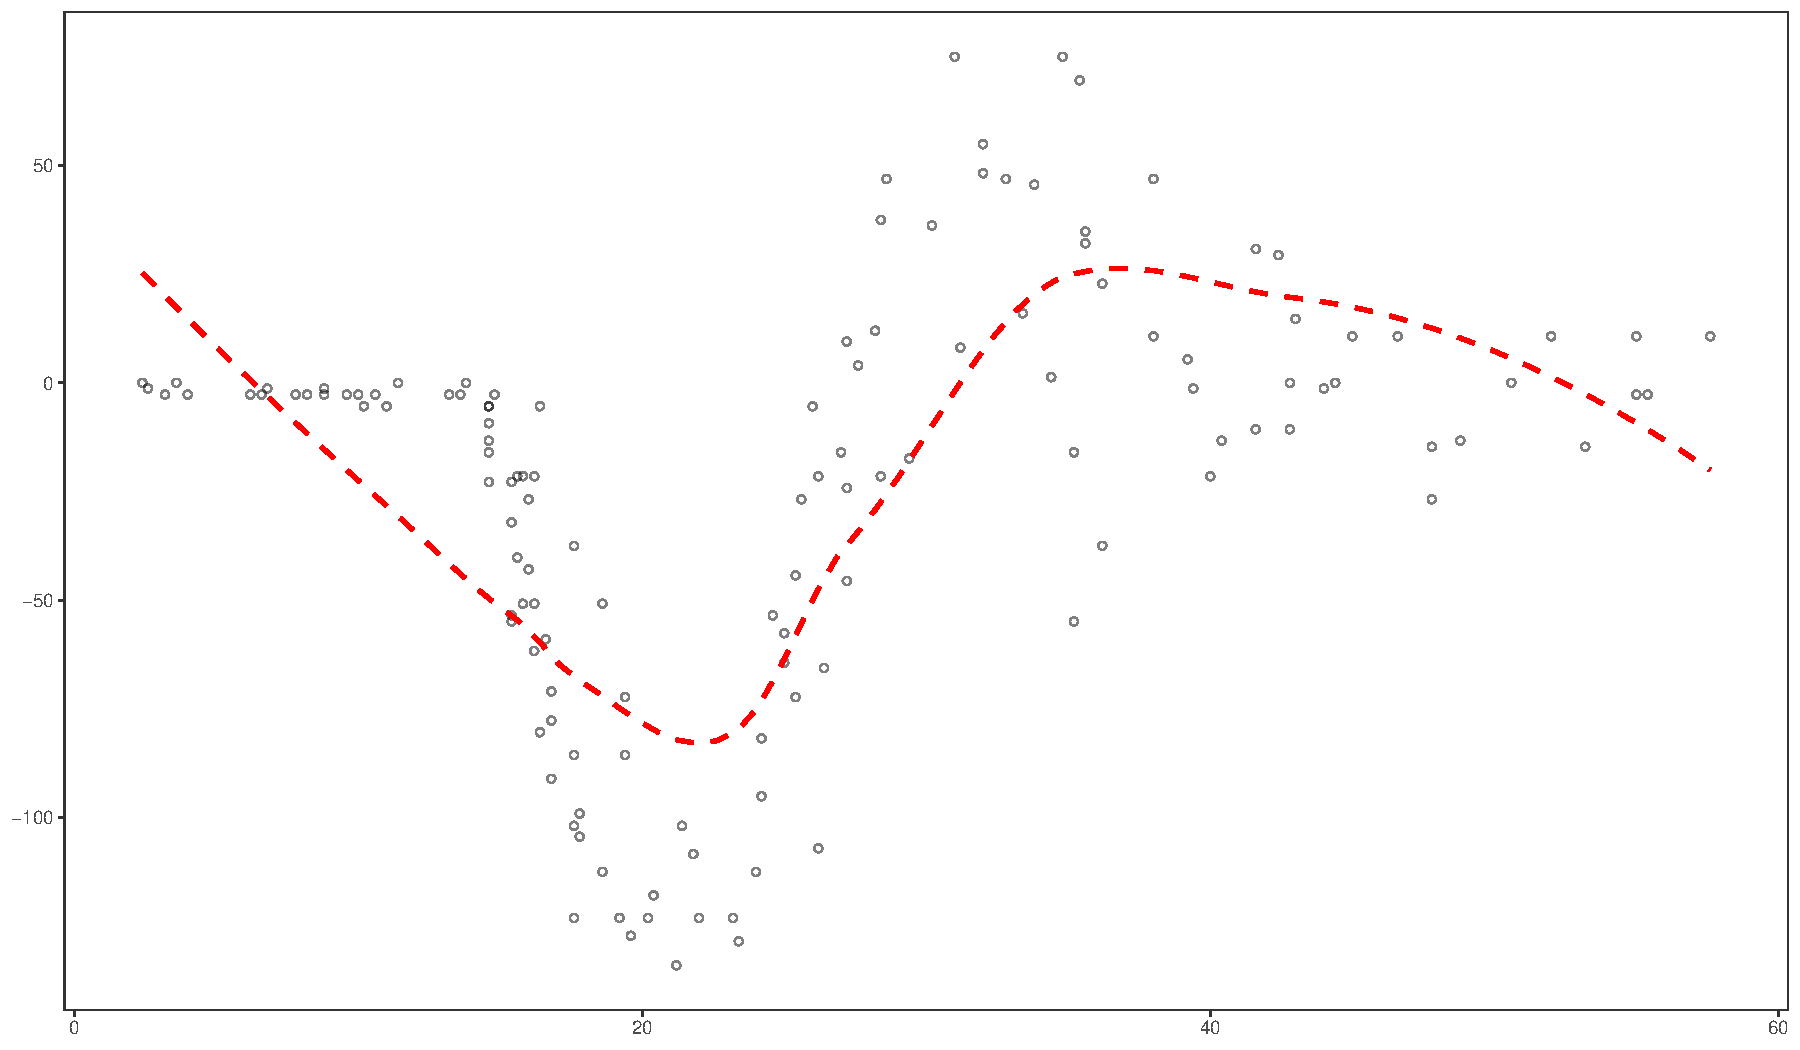
\includegraphics[scale=0.25]{figures/fig_1c.pdf}
  \\
  \tiny
  Source: motorcycle data from \url{https://www.stata-press.com/data/r12/r.html}
\end{figure}

\end{frame}

%----------------------------------------------------------------------%

\begin{frame}
\frametitle{How to estimate $f(.)$}


\begin{itemize}
  \item Linear vs Local Polynomial Regression
\end{itemize}

\begin{figure}[H] \centering
  \centering
  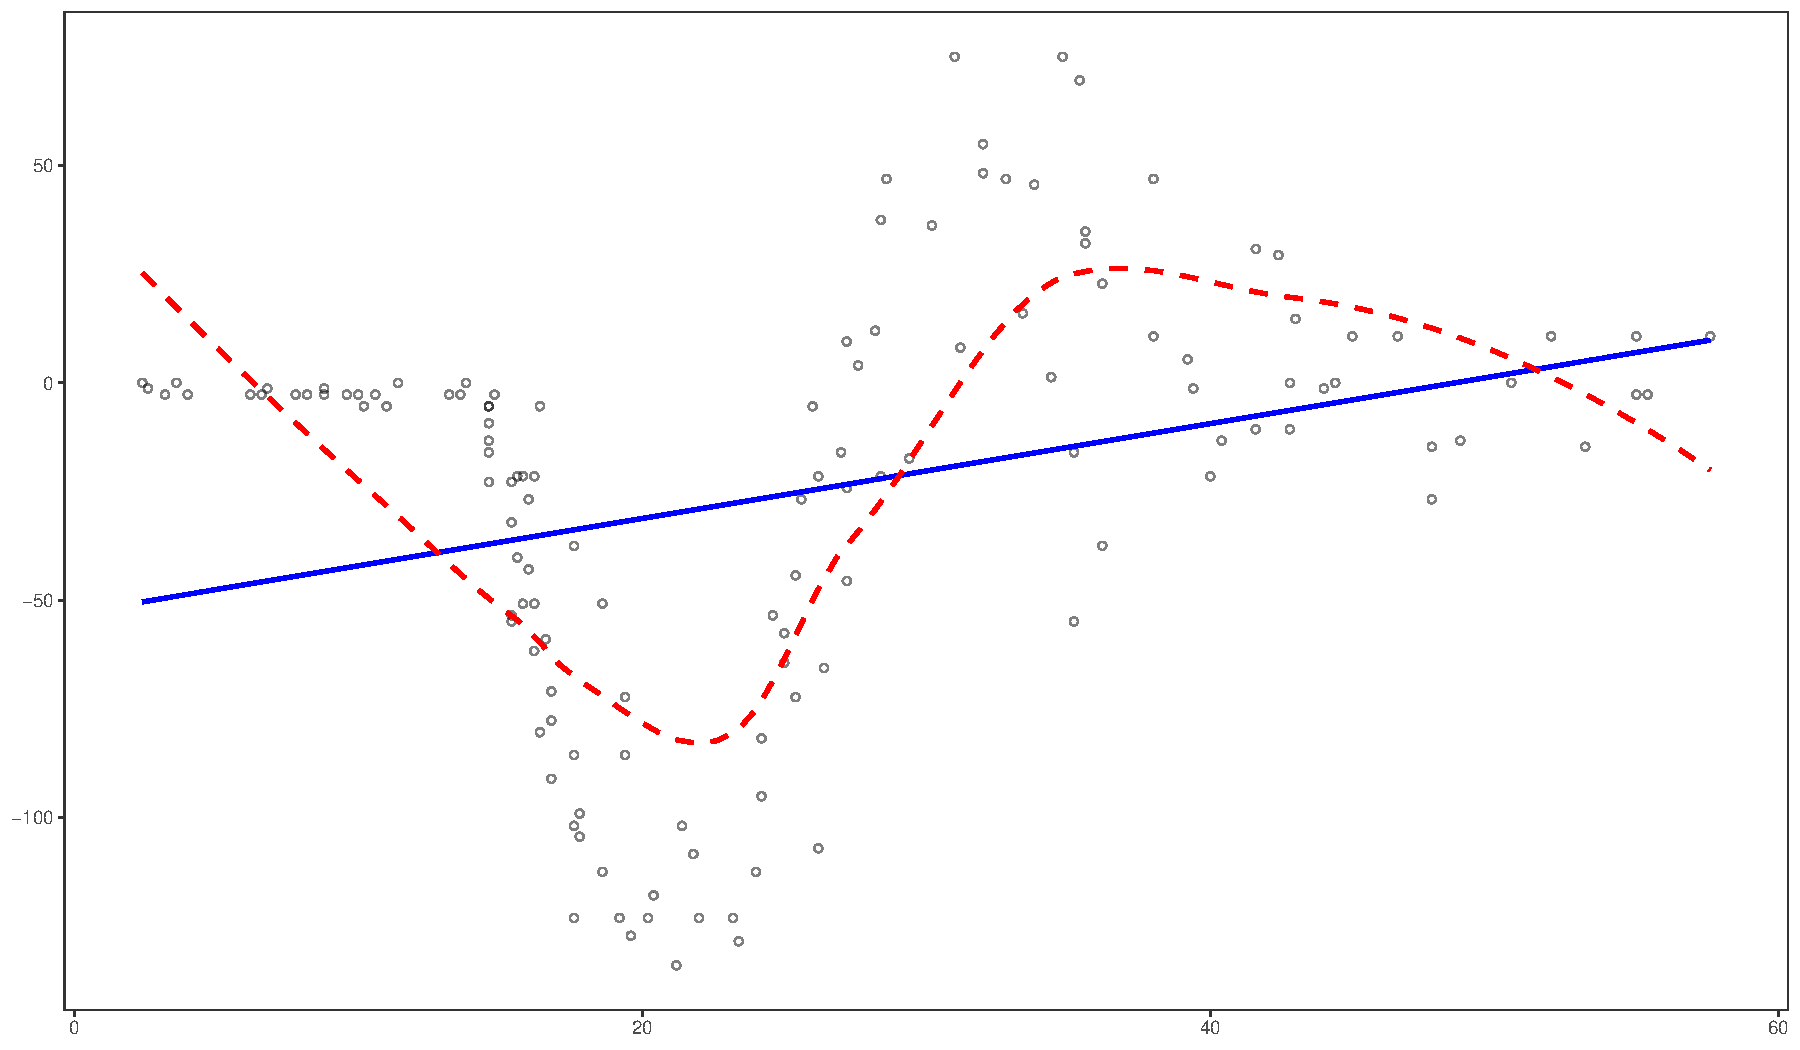
\includegraphics[scale=0.25]{figures/fig_1d.pdf}
  \\
  \tiny
  Source: motorcycle data from \url{https://www.stata-press.com/data/r12/r.html}
\end{figure}


\end{frame}
%----------------------------------------------------------------------%


\begin{frame}
\frametitle{Accuracy, complexity and interpretability}

\begin{figure}[H] \centering
  \centering
  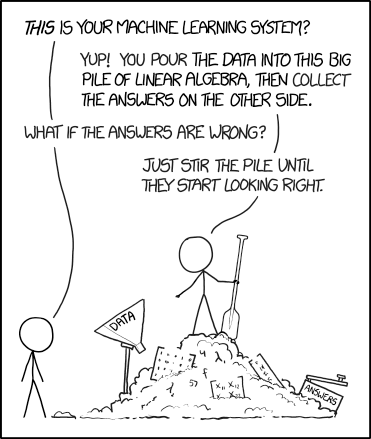
\includegraphics[scale=0.35]{figures/machine_learning}
  \\
  \tiny
  Source: \url{https://imgs.xkcd.com/comics/machine_learning.png}
\end{figure}

\end{frame}
%----------------------------------------------------------------------%


\begin{frame}
\frametitle{Accuracy, complexity and interpretability}

Recall the problem of interpretation in

\begin{align}
Y=\beta_1+\beta_2 X+\beta_3 X^2+u
\end{align}

\begin{itemize}
  \item We have lost the interpretation of $\beta_2$ as a marginal effect
  \item In a non-linear model the interpretations are no longer trivial
  \item Machine learning: we quickly lose interpretability in predictive quality post
  \item Is this a problem?
\end{itemize}
\end{frame}

%----------------------------------------------------------------------%
\begin{frame}
\frametitle{Accuracy, complexity and interpretability}

\begin{itemize}
  \item Is this a problem?
\end{itemize}

\bigskip

\begin{figure}[H] \centering
  \centering
  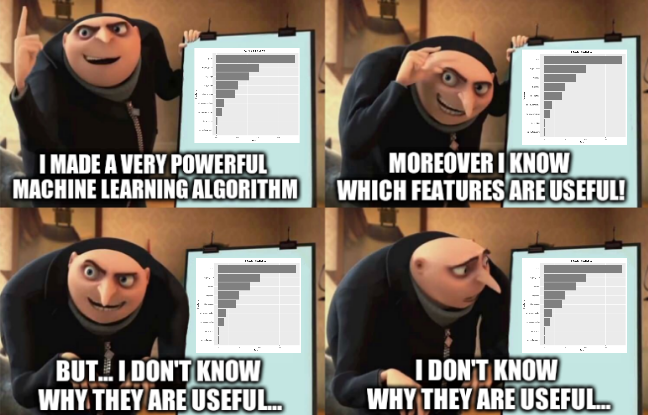
\includegraphics[scale=0.3]{figures/feature_importance.png}
  \\
  \tiny
  Source: \url{shorturl.at/gm013}
  \end{figure}

\end{frame}


%----------------------------------------------------------------------%
\begin{frame}
\frametitle{Supervised vs Unsupervised}


\begin{itemize}
  \item Supervised Learning 
  \begin{itemize}
    \item for each predictor $x_i$ a 'response' is observed $y_i$.
    \item everything we have done in econometrics is supervised
  \end{itemize}
\end{itemize}

\bigskip
\begin{figure}[H] \centering
  \captionsetup{justification=centering}
  
    \centering
    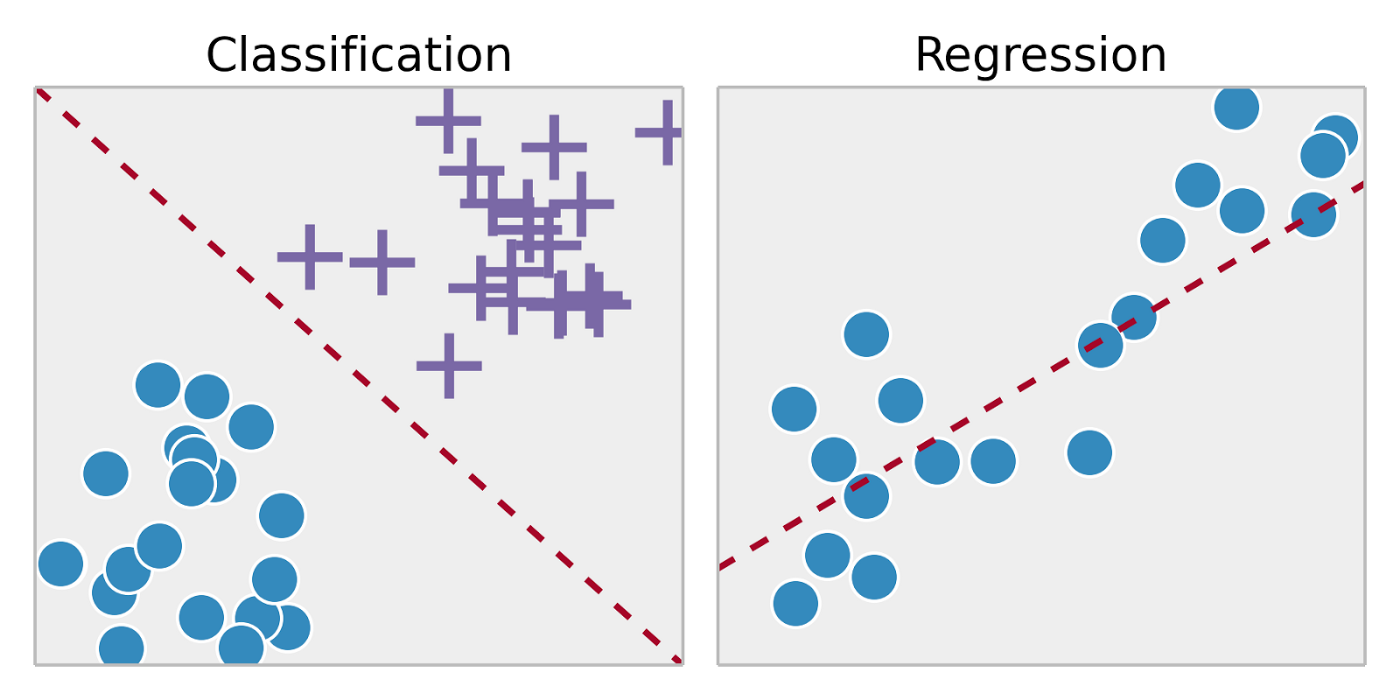
\includegraphics[scale=0.15]{figures/supevised}
  \\
  \tiny
  Source: \url{shorturl.at/opqKT}
  \end{figure}
  
\end{frame}


%----------------------------------------------------------------------%
\begin{frame}
\frametitle{Supervised vs Unsupervised}

\begin{itemize}
  \item Unsupervised Learning 
  \begin{itemize}
    \item observed $x_i$ but no response. 
    \item example: cluster analysis
  \end{itemize}
  \end{itemize}

\bigskip
    \begin{figure}[H] \centering
  
    \centering
    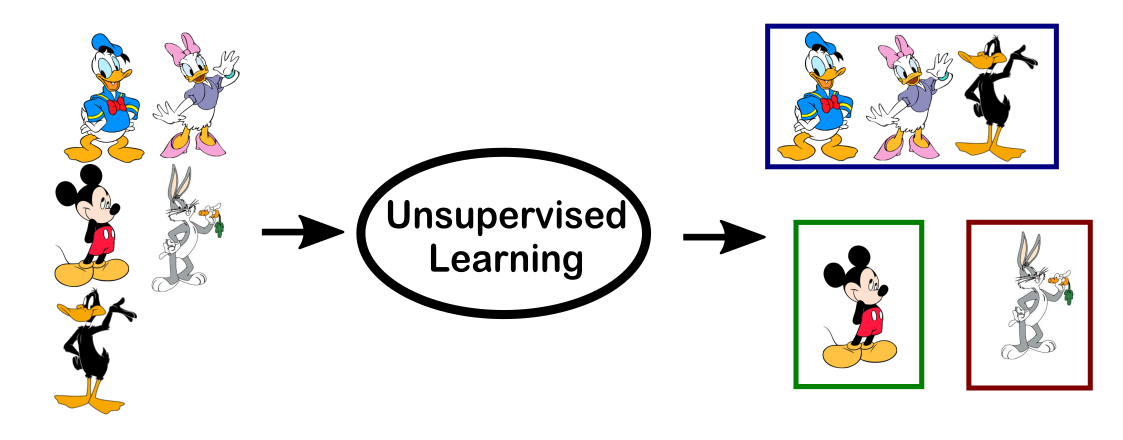
\includegraphics[scale=0.2]{figures/unsupevised}
  \\
  \tiny
  Source: \url{shorturl.at/opqKT}
\end{figure}


\end{frame}
%----------------------------------------------------------------------%
\section{Recap}
\begin{frame}
\frametitle{Recap}

\begin{itemize} 
    \item We start shifting paradigms
    \medskip
    \item Tools are not that different (so far)
    \medskip
    \item Decision Theory: Risk with square error loss $\rightarrow$ MSE
    \medskip
    \item Objective minimize the reducible error
    \medskip
    \item Irreducible error our unknown bound
    \medskip
    \item Machine Learning best kept secret:  some bias can help lower MSE
\end{itemize}
\end{frame}

%----------------------------------------------------------------------%

\section{If there's time left}

\begin{frame}
\frametitle{Next}
  
  \begin{itemize} 
  \item  Next Class: OLS, Geometry, BLUE, BLUP
  \bigskip
  \item  GitHub Demo
  \bigskip
  \item Questions about software installation
  \medskip
    \begin{itemize} 
      \item  \texttt{R} and \texttt{RStudio}
      \medskip
      \item \texttt{Conda}? 
    \end{itemize}
  \end{itemize}


\end{frame}

%----------------------------------------------------------------------%

\begin{frame}
\frametitle{Further Readings}

\begin{itemize}
  \item Casella, G., \& Berger, R. L. (2002). Statistical inference (Vol. 2, pp. 337-472). Pacific Grove, CA: Duxbury.
  \bigskip
  \item James, G., Witten, D., Hastie, T., \& Tibshirani, R. (2013). An introduction to statistical learning (Vol. 112, p. 18). New York: springer.
  \bigskip
  \item Friedman, J., Hastie, T., \& Tibshirani, R. (2001). The elements of statistical learning (Vol. 1, No. 10). New York: Springer series in statistics.
  \bigskip
  \item Mullainathan, S. and Spiess, J., 2017. Machine learning: an applied econometric approach. Journal of Economic Perspectives, 31(2), pp.87-106.
  

\end{itemize}

\end{frame}

%----------------------------------------------------------------------%
\end{document}


